\documentclass[11pt,ngerman,parskip=half]{scrartcl}

\usepackage[utf8]{inputenc}
\usepackage[T1]{fontenc}
\usepackage{libertine}
\usepackage{babel}
\usepackage{graphicx}
\usepackage[style=authoryear-icomp,loccittracker=context]{biblatex}
\usepackage[thresholdtype=lines,threshold=2]{csquotes}
\usepackage{xpatch}
\usepackage{hyperref}
\usepackage{float}
\usepackage{mathtools}

\addbibresource{src/library.bib}
\author{}
\titlehead{
  \begin{center}
     
\includegraphics[width=0.7\textwidth]{src/img/htw-logo.pdf}
  \end{center}
}
\title{Gehirn-Computer-Schnittstellen in Neuroprothesen}

\begin{document}
\maketitle
\begin{tabular}{ll}
  Fachbereich: & 4 (Informatik, Kommunikation und Wirtschaft) \\
  Studiengang: & Angewandte Informatik (SoSe2018)             \\
  Seminar:     & B15 Gesellschaftliche Aspekte der Informatik \\
  Dozentin:    & Prof.-Dr. Christin Schmidt                   \\
\end{tabular}

\begin{tabular}{ll}
  Gruppe: & 5 \\
\end{tabular}

\begin{tabular}{lll}
  Gruppenmitglied        & Matrikelnummer & Kapitel\\
  Louis Knorn            & 566546         & 1\\
  John-Kevin Gold        & 566538         & 2\\
  Jeremy Etienne Seipelt & 566847         & 3\\
  Kathrin Klocke         & 514403         & 4\\
\end{tabular}

\newpage
\tableofcontents
\newpage
\listoffigures
\newpage
\listoftables
\newpage

\section{Funktionsweise der Gerätetechnik von Gelenkarmrobotern}
\subsection{Einführung}
\label{subsec:Einführung}
Der Artikel \enquote{Neuroprothese: Gelähmter steuert Roboterarm mit bloßer
Vorstellungskraft} aus dem Jahr 2015 beschreibt, wie ein Mensch einen
Industrieroboter-ähnlichen Gelenk- bzw. Knickarmroboter mittels eines
Brain-Computer-Interface steuert
\parencite[vgl.][]{merkelt_neuroprothesen:_2015}. Die Idee, verlorene oder
gelähmte Gliedmaßen durch Roboterarme zu ersetzen, ist allerdings nicht völlig
neu. Bereits im Jahr 1979 veröffentlichten Guittet u. a. eine Fallstudie, die
eine vergleichbare Anwendung untersuchte. Man bezeichnete einen solchen
Roboterarm auch als Telethese, allerdings wurde der Arm damals durch einfache
Kopfbewegungen kontrolliert \parencite[vgl.][]{guittet_spartacus_1979}.

\begin{figure}[H]
  \centering
  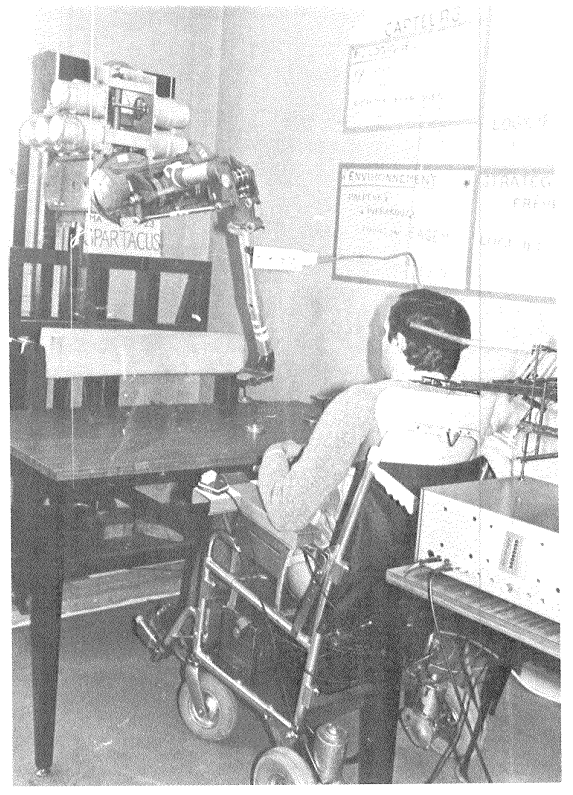
\includegraphics[width=0.6\textwidth]{src/img/spartacus.png}
  \caption{Knickarmrobotersteuerung durch Kopfbewegungen}
  \label{img:spartacus}
  \parencite[][84]{guittet_spartacus_1979}
\end{figure}
\newpage

Nachdem im ersten Kapitel der Gruppenarbeit die Funktionsweise von BCI
erläutert wurde, beschäftigt sich der folgende Abschnitt mit der
Gerätetechnik eines Gelenkarmoboters sowie Begriffen und Grundlagen der
Robotik im Allgemeinen. Die Gerätetechnik gehört zu den Kernkomponenten in
einem Robotersystem und beinhaltet technische Elemente für Kinematik,
Sensorik und Aktorik. Zu den weiteren Kernkomponenten, die im Rahmen der
Belegarbeit nicht weiter behandelt werden, zählen:
\begin{itemize}
  \item Steuerung (z.B. Rechnerkopplung, Interpolation)
  \item Programmierung (z.B. Punkt- und Bahnsteuerung, Prozessbeschreibung)
  \item Prozessführung (Geometrie- und Technologiedatenverarbeitung, Steuer-
        und Regelstrategie)
  \item Endeffektor (z.B. Greifer, Werkzeuge)
\end{itemize}
\parencite[vgl.][40]{hesse_taschenbuch_2016}

Der Begriff Robotik ist laut DIN definiert als:
\blockquote[{\cite[DIN EN ISO 8373, zitiert nach][39]
{hesse_taschenbuch_2016}}]{Robotertechnik, zu der man Entwurf und
Berechnung, Herstellung, Steuerung von Robotern, Einsatz in Standard- und
Problemlösungen, Erforschung von Steuerungsvorgängen bei Mensch und Maschine,
Sensoren und Endeffektoren sowie deren Anwendung zählt}.
Roboter können nach verschiedenen Kriterien, wie Anwendungsbereich,
Einsatzgebiet, Ausführung und Aufgaben, gruppiert werden
\parencite[vgl.][25\psq]{hesse_taschenbuch_2016}. Die VDI-Richtlinie 2860
beschreibt Industrieroboter beispielsweise wie folgt:
\blockquote[{\cite[VDI-Richtlinie 2860, zitiert nach][16]
{weber_industrieroboter:_2017}}]{Industrieroboter sind universell
einsetzbare Bewegungsautomaten mit mehreren Achsen, deren Bewegungen
hinsichtlich Bewegungsfolge und Wegen bzw. Winkeln frei programmierbar (d.h.
ohne mechanischen Eingriff vorzugeben bzw. änderbar) und gegebenenfalls
sensorgeführt sind. Sie sind mit Greifern, Werkzeugen oder anderen
Fertigungsmitteln ausrüstbar und können Handhabe- oder andere
Fertigungsaufgaben ausführen}.

Roboter, insbesondere Industrieroboter, können demnach auch als
Handhabungsgeräte bzw. -technik betrachtet werden.
Abbildung~\ref{img:einteilung-von-handhabungsgeraeten} zeigt, dass
Handhabungsgeräte primär in manuell gesteuerte oder programmgesteuerte Geräte
eingeteilt werden können. Es gibt darüber hinaus aber auch Mischformen in der
Robotik, z.B. beim Serviceroboter. Dieser ist ein Hybrid aus Industrieroboter
und Manipulator, welcher Dienstleistungen für den Menschen erbringt.
Serviceroboter reagieren auf menschliche Anweisungen (manuelle Steuerung)
führen Teilaufgaben aber auch automatisch bzw. programmgesteuert aus.
\parencite[vgl.][15--17]{weber_industrieroboter:_2017}

\begin{figure}[H]
  \centering
  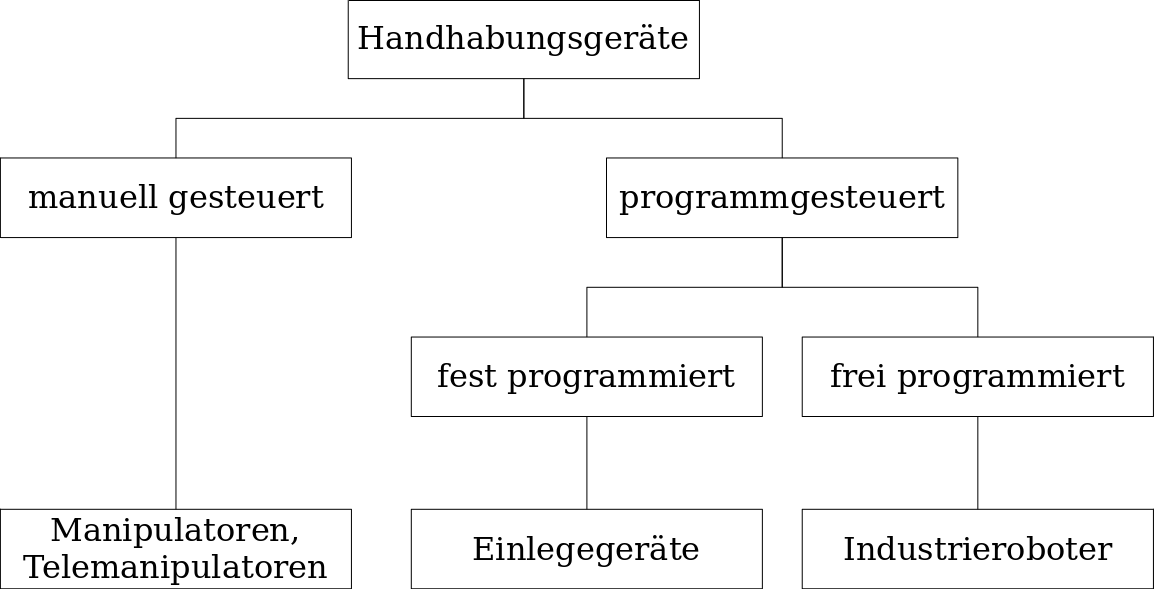
\includegraphics[width=0.7\textwidth]{src/img/einteilung-von-handhabungsgeraeten.png}
  \caption{Einteilung von Handhabungsgeräten}
  \label{img:einteilung-von-handhabungsgeraeten}
  \parencite[][16]{weber_industrieroboter:_2017}
\end{figure}

\subsection{Kinematik}
\label{subsec:Kinematik}
Die Anordnung der Armteile und Gelenke bestimmt die kinematische Struktur
eines Roboters, hierbei unterscheidet man hauptsächlich zwischen serieller
Kinematik und Parallelkinematik. Roboter die aus einer Aneinanderreihung von
Armteilen bestehen, welche wiederum durch Gelenke bzw. Achsen verbunden sind,
ordnet man der seriellen Kinematik zu. Das letzte Armteil in einer solchen
Anordnung, kann auch als Effektor bzw. Endeffektor bezeichnet werden. Hierbei
handelt es sich um das Teil des Roboters, welches in Kontakt mit der Umgebung
tritt, um z.B. Objekte zu greifen. Bei der Parallelkinematik hingegen sind
mehrere Schub- oder Drehgelenke mit dem Effektor verbunden und wirken direkt
auf diesen. Der Gelenkarmroboter weist eine serielle Kinematik auf. Die
kinematische Struktur eines Roboters bestimmt wiederum seinen Freiheits- bzw.
Getriebefreiheitsgrad. \parencite[vgl.][17--20]{weber_industrieroboter:_2017}

Der Freiheitsgrad \textit{f} beschreibt
\textquote[{\cite[][18]{weber_industrieroboter:_2017}}]{[...] die Anzahl der
möglichen unabhängigen Bewegungen (Verschiebungen, Drehungen) eines starren
Körpers gegenüber einem Bezugssystem}. Es gibt hierbei zwei wesentliche
Grundbewegungen, die Translation (Gleit- oder Verschiebebewegung) und die
Rotation (Drehbewegung). Bei der Translation bewegt sich der Körper
theoretisch ohne sich selbst zu drehen (starr) entlang einer oder mehrerer
Raumachsen (x-, y- und z-Achse). Bei der Rotation hingegen dreht sich der
Körper um einen bestimmten Mittelpunkt bzw. um eine bestimmte Achse, die
innerhalb oder außerhalb des Körpers liegen kann.
\parencite[vgl.][53\psq]{schunke_funktionelle_2014}

Abbildung~\ref{img:translation-rotation} stellt die Freiheitsgrade am
Beispiel der Bewegungsmöglichkeiten eines Tennisballs im Raum dar.
\begin{figure}[H]
  \centering
  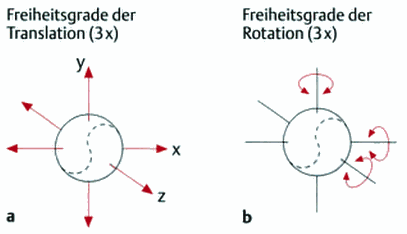
\includegraphics[width=0.6\textwidth]{src/img/translation-rotation.png}
  \caption{Translation (a) und Rotation (b)}
  \label{img:translation-rotation}
  \parencite[][53]{schunke_funktionelle_2014}
\end{figure}

Der Getriebefreiheitsgrad F gibt an,
\textquote[{\cite[][18]{weber_industrieroboter:_2017}}]{[...] wie viele
unabhängig voneinander angetriebene Achsen zu einer eindeutigen Bewegung des
Roboterarms führen}. Bei Gelenkarmrobotern mit sechs Achsen (F=6), kann der
Effektor durch geschickte Anordnung der Gelenke, den maximalen Freiheitsgrad
f=6 erreichen. Roboter können generell aber auch mit mehr als sechs Achsen
(F>6) konstruiert werden, dies bezeichnet man als redundante Kinematiken.
Hierdurch erzielt man auf Kosten eines erhöhten Steuerungsaufwands eine
Verbesserung der Feinbewegungen.
\parencite[vgl.][18]{weber_industrieroboter:_2017}

Abbildung~\ref{img:KR-AGILUS-sixx} zeigt die Drehrichtung der Roboterachsen des
Gelenkroboters KUKA KR AGILUS sixx.
\begin{figure}[H]
  \centering
  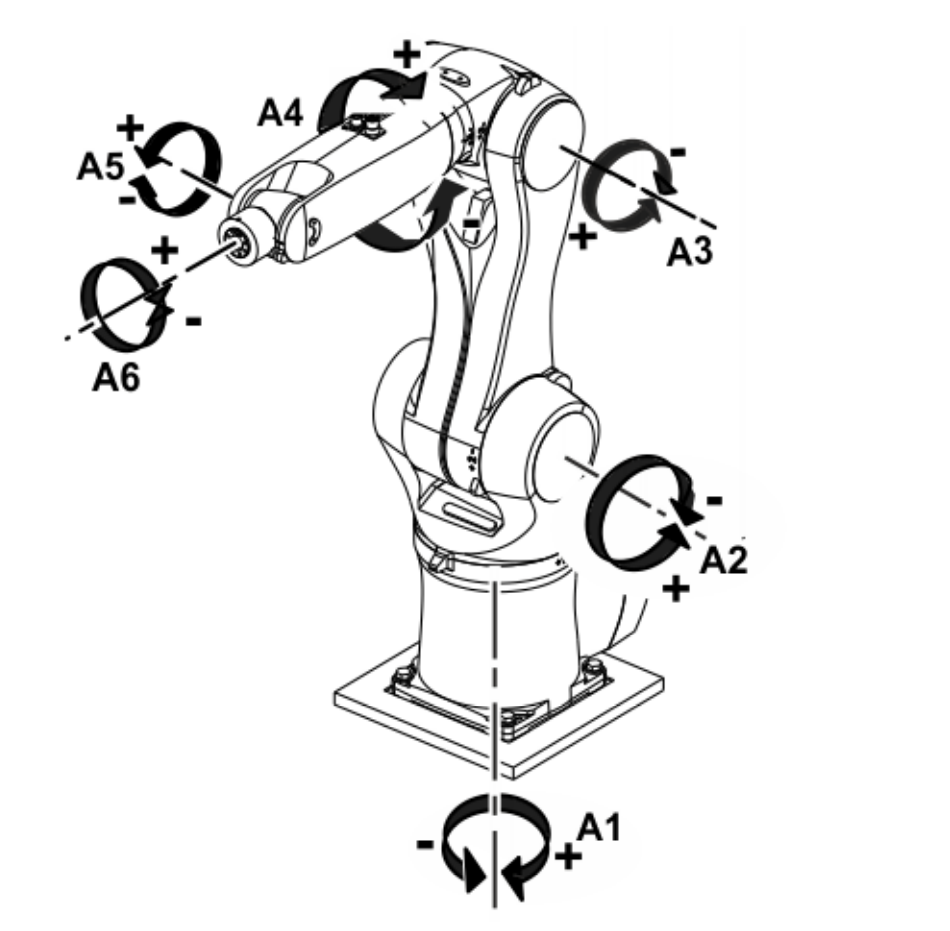
\includegraphics[width=0.5\textwidth]{src/img/KR-AGILUS-sixx.png}
  \caption{KR AGILUS sixx}
  \label{img:KR-AGILUS-sixx}
  \parencite{kuka_gmbh_kr_2018}
\end{figure}

\subsection{Aktorik}
\label{subsec:Aktorik}
Gelenkmodule und Achsverbindungen werden durch die Aktorik eines Roboters
angetrieben und ermöglichen somit die Bewegung des Effektors. Der Aktor hat
demnach die Aufgabe eine Achse von einer Position auf eine andere zu bewegen,
hierzu gibt es vier typische Betriebszustände:
\begin{itemize}
  \item Antrieb und Beschleunigung im Rechtslauf
  \item Abbremsung im Rechtslauf
  \item Antrieb und Beschleunigung im Linkslauf
  \item Abbremsung im Linkslauf
\end{itemize}

Zu den wesentlichen Gruppen in der Aktorik gehören pneumatische oder
hydraulische Aktoren (z.B. doppeltwirkende Zylinder oder Druckluftmotoren)
sowie elektrische Aktoren (z.B. bürstenbehaftete und bürstenlose
Gleichstrommaschinen). Jede Gruppe hat ihre individuellen Vor- und Nachteile,
weshalb in einem Robotersystem, und so z.B. auch bei einem Gelenkarmroboter,
verschiedene Kombinationen von Aktoren zum Einsatz kommen können. Generell
lässt sich festhalten, dass pneumatische und hydraulische Aktoren die
höchsten Kräfte erzielen und daher sehr hohe Geschwindigkeiten erreichen
können, allerdings erreichen sie nicht die hohe Positioniergenauigkeit von
elektrischen Aktoren.
\parencite[vgl.][63--79]{hesse_taschenbuch_2016}

Neben dem eigentlichen Antrieb bzw. Motor sind auch Getriebe teil der Aktorik
in einem Roboter. Getriebe sind notwendig, da die Bewegungen der Aktoren
nicht immer direkt den Anforderung des mechatronischen Systems entsprechen.
Sie dienen allgemein der Übertragung und Umformung von Bewegungen sowie von
Kräften, mittels der Änderung von Drehmomenten, -richtungen oder der
Umsetzung einer Drehbewegung in eine Linearbewegung. Auch hier gibt es viele
verschiedene Bauformen, deren Anwendung je nach Anforderung variiert, z.B.
Kugelumlaufspindeln, Planetengetriebe, Kegelradgetriebe oder Zahnriemengetriebe.
\parencites[vgl.][121\psq]{maccloy_robotertechnik:_1989}
[][89--96]{hesse_taschenbuch_2016}

\subsection{Sensorik}
\label{subsec:Sensorik}
Die Sensorik in einem Robotersystem ermittelt inner- und außerhalb des
Systems vorliegende Informationen. Dies ist erforderlich um die komplexen
Bewegungsabläufe in einer nur teilweise bestimmbaren Umwelt auszuführen. Die
Robotik stützt sich dabei häufig auf Erkenntnisse aus der Bionik\footnote{
Die Bionik erforscht wie biologische Phänomene auf technische Systeme
übertragen werden können. \parencite{feess_definition:_2018}} und man
unterscheidet primär zwischen internen (interozeptiven bzw. propriozeptiven)
und externen (exterozeptiven) Sensoren. Interozeptive Sensoren messen interne
Zustände wie Motorgeschwindigkeit, Ladezustand oder Greifkraft und
exterozeptive Sensoren ermitteln Informationen aus der Umgebung, z.B. zur
Entfernungsmessung von Objekten. Nutzt ein Sensor dabei nur die Energie bzw.
Signale aus der Umgebung, bezeichnet man ihn auch als passiven Sensor (z.B.
Kameras oder Kontaktsensoren). Aktive Sensoren hingegen senden Energie aus
und messen die Reaktion der Umgebung darauf (z.B. Laser- \&
Ultraschallscanner sowie Infrarotsensoren).
\parencites[vgl.][23\psq]{hertzberg_mobile_2012}[][73]
{kruse_mehrobjekt-zustandsschatzung_2013}[][97]{hesse_taschenbuch_2016}

Zu den wesentlichen Aufgaben der Sensorik zählen:
\textquote[{\cite[][97]{hesse_taschenbuch_2016}}]{
  \begin{itemize}
    \item Bewegungsüberwachung (z.B. Abgleich- und Justiervorgänge)
    \item Bewegungssteuerung (z.B. Konturverfolgung)
    \item Kraftsteuerung (z.B. Einpressen, Zusammenstecken)
    \item Sensorgesteuertes Erreichen einer Zielposition (unbekannte Position
          und Orientierung eines Teils)
    \item Programmablaufkontrolle (z.B. selektive Montage)
    \item Überwachung von Endeffektoren (z.B. Greifkraft, Rutschsensor)
  \end{itemize}
}

Zu den wichtigsten Sensoren gehören Positionssensoren,
Beschleunigungssensoren und Sensoren zur Kräftemessung. Positionssensoren
ermitteln die Position bewegter Komponenten wie dem Endeffektor und lassen sich
z.B. durch inkrementale Weg- und Winkelgeber, Resolver oder elektrische Kompasse
realisieren. Zur optischen Positionsmessung gibt es neben Kameras eine Vielzahl 
von Lasersensoren mit unterschiedlichen Funktionsweisen wie
Laserlaufzeitmessung, Lasermodulation, -triangulation oder -interferometrie.
Beschleunigungssensoren messen Beschleunigungen und Rotationsraten, um die
aktuelle Position und Orientierung eines betrachteten Körpers ausgehend von
einer bestimmten Startposition zu berechnen. Hier kommen z.B. elektrische
oder optische Gyroskope zum Einsatz. Zur Kräftemessung werden in der modernen
Robotik Kraft-Moment-Sensoren eingesetzt, welche in der Regel alle drei
Raumkräfte und -momente messen. Die Messung erfolgt dabei über
piezoelektrische Elemente oder Dehnmessstreifen.
\parencite[vgl.][98--117]{hesse_taschenbuch_2016}

\subsection{Fazit}
\label{subsec:Fazit}
Roboter sind höchst komplexe mechatronische Systeme, die primär aufgrund
ihrer industriellen Nutzung weiterentwickelt wurden. Es hat sich gezeigt,
dass der Effektor eines Gelenkarmroboters im Vergleich zu anderen
kinematischen Strukturen den höchsten Freiheitsgrad erreichen kann. Daraus
begründet sich auch der geeignete Einsatz als Telethese. Allerdings konnten
im Rahmen der Belegarbeit viele wichtige Fragen, wie beispielsweise zur
Steuerung, Prozessführung oder den Endeffektoren, nicht geklärt werden. In
Anbetracht der Komplexität von Robotersystemen stellt sich auch die Frage
nach sicherheitstechnischen Anforderungen, insbesondere wenn solche Systeme
als Prothesen genutzt werden. Während bei stationären Industrierobotern z.B.
umzäunte Sperrbereiche eingerichtet werden können, bestünde im Fall von
Fehlfunktionen bei einem mobilen Roboterarm die Gefahr Lebewesen oder Objekte
im unmittelbaren Umfeld oder den Anwender selbst zu verletzen.

\newpage
\printbibliography[heading=bibintoc]

\end{document}
